
In this section we'll go over several commands that can be very useful for automating certain bits of code.

\subsection{Grouped Command Execution}
One of the easiest ways we can repeat a certain command for different groups of observations is with the \st{bysort} prefix.
This prefix lets us run the command we use it with for every group defined by a variable separately.
In my experience it's mostly useful for generating variables in programming,
but it can also be used as a quick and dirty way to compare variables across groups.
We can use the prefix like so: \st{bysort varlist: command},
where \st{varlist} is a list of the variables -- or a single variable --identifying the different groups,
and \st{command} is the command we would like to run.
Note that \st{bysort varlist:} is equivalent to using \st{by varlist, sort:}.
The \st{by} prefix does not work without sorting the data, so it is generally easier to just use \st{bysort}.
\cref{lst:sort} provides an example.

\begin{listing}[htp]
\caption{bysort.do}\label{lst:sort}
\inputst{bysort.do}
\end{listing}

\subsection{Conditionals}
Conditionals, or if-statements, are where the real fun stuff begins.
To put it simply,
they allow us to differentiate our code based on anything we can turn into an expression that evaluates to true or false.
Stata recognises two types of if-statements: one as a command suffix,
and one for programming.
In this section,
we'll first go over expressions before we move on to the two types of if-statements.

\subsubsection{Expressions}
When we use conditionals,
we set requirements that must hold for code to be executed.
An expression can then be seen as a check whether these requirements are fulfilled.
An expression always evaluates to true or false:
the requirements are met, or they are not.
In programming, we refer to a data type that has either the value ``true'' or ``false'' as a \emph{boolean}.
An evaluated expression is precisely that.
In programming,
true and false are often represented by $1$ and $0$, respectively.
This is also the case in Stata:
if we look at dummy variables,
for example,
they function in much the same way.
A dummy variable for gender is often coded in such a way that it represents either male or female,
such as a variable \st{female} with value $1$ for females and value $0$ for males.

Expressions are much like mathematical equations,
in that they have a left-hand side,
a relational operator,
and a right-hand side.
Based on the relational operator,
the left-hand side is compared to the right-hand side,
and the expression is evaluated to be true or false.
Let's take a look at an example.
Suppose we have two scalars, $a$ and $b$,
and want to check whether these are equal to one another.
First, we need to have these scalars defined.
Let's say that $a=3$ and $b=\pi$:
\begin{minted}{stata}
// define scalars
sca a = 3
sca b = c(pi)

// inspect the values of the scalars
di "Scalar a holds value " a
di "Scalar b holds value " b
\end{minted}
We then want Stata to tell us whether $a=b$:
\begin{minted}[firstnumber=9]{stata}
// show whether a and b are equal
di a == b
\end{minted}
Of course, clever as we are, we know this to be false.
This expression should therefore evaluate to false, i.e., $0$.
When we run this code, we see that, indeed, the last command returns $0$ (see \cref{fig:exp}).

\begin{figure}[tbp]\centering
    \caption{Stata output for expression code}\label{fig:exp}
    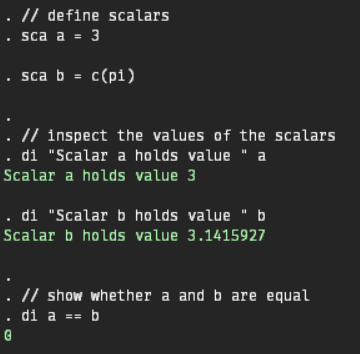
\includegraphics[width=0.5\textwidth]{expression.png}
\end{figure}

Of course, we don't always want to know whether things are equal to one another.
Luckily, there are more relational operators than just \st{==} (equals).
To see the full list of available operators,
type \st{help operator} in the command window.
Furthermore, we may want to set more than one requirement.
Luckily, we can combine multiple requirements using logic operators -- also listed in \st{help operator}.

Suppose we now want to know whether $a \leq b$.
We could then tell Stata to tell us whether $a = b$ \emph{or} $b > a$ is true:\footnote{%
Of course, this can also be achieved using a single $\leq$ operator,
but for the sake of the example I don't do that here.}
\begin{minted}[firstnumber=12]{stata}
// show whether a and b are equal, or b is larger than a
di a == b | b > a
\end{minted}
As $\pi > 3$, this will evaluate to true.
Try for yourself using the code in \cref{lst:expression}!

\begin{listing}[htp]
\caption{expression.do}\label{lst:expression}
\inputst{expression.do}
\end{listing}


\subsubsection{Command suffix if}
The command suffix if statement is the simpler of the two.
By adding an if-statement to the end of a command (but before the options!) we tell Stata to only use the specified subset of our data.
You've likely done this before,
but let's go over an example.
First, we'll use one of Stata's example datasets:
\begin{minted}{stata}
// load example dataset
sysuse auto, clear

// inspect available variables
describe
\end{minted}

Here, the variable \st{foreign} is a dummy variable indicating whether the origin of a car is foreign (value $1$), or domestic (value $0$).
Suppose now we want some descriptive statistics,
but only for imported cars.
We do this by adding an if-statement to the \st{summarize} command that evaluates to true only for foreign cars.
Before we do this,
recall the way Stata handles true/false data:
using the values $1$ and $0$.
When ``splitting'' our data based on a dummy variable,
we can exploit this to write very compact if-statements,
like so:
\begin{minted}[firstnumber=7]{stata}
// summary statistics of foreign cars
sum if foreign
\end{minted}
As the dummy already indicates whether it is true that the car is foreign (by taking a value of $1$),
we no longer have to add a relational operator.
Of course, we could do so, but it would be redundant;
we would effectively telling Stata \emph{do }x \emph{if it is true that }y \emph{is true}.
For illustrative purposes,
the code to do so here would be \st{sum if foreign == 1}.

Note that we can use this same ``trick'' when generating our own dummy variables.
Suppose we want to create a dummy indicating whether a car in the dataset is expensive,
say, has a price equal to or over 10,000\$.\footnote{%
I'm just going to assume the prices in this dataset are in dollars,
as the currency isn't really mentioned in the dataset.}
The way I used to do this is as follows:
\begin{minted}{stata}
// generate dummy for expensive cars
gen expensive = 1 if price >= 10000
replace rexpensive = 0 if price < 10000
\end{minted}
But we could actually just write
\begin{minted}[firstnumber=10]{stata}
// generate dummy for expensive cars
gen expensive = price >= 10000
\end{minted}
to get exactly the same variable!
See for yourself using \cref{lst:suffix}.

\begin{listing}[htp]
\caption{suffix-if.do}\label{lst:suffix}
\inputst{suffix-if.do}
\end{listing}

\subsubsection{Programming if}
Stata's programming if-statements have a multitude of uses.
They allow us to execute bits of code only if a specified expression is true.
For a single command,
the syntax is as follows:
\begin{minted}{stata}
if expression command
\end{minted}
where the expression works in the same way as in the suffix if-statement.
In programming if-statements,
you probably won't be using variable names,
but rather locals or scalars that you defined previously.
Of course,
you are free to do as you like:
locals and scalars can also be used in suffix if-statements,
and variables can be used in programming if-statements,
although the latter will generally include an observation number to identify a specific value.\footnote{I.e.\ by writing \st{varname[number]} instead of simply \st{varname}}

We can also include multiple commands in a single if-statement.
The syntax for this is slightly different:
\begin{minted}{stata}
if expression {
    command1
    command2
    ...
}
\end{minted}
Should the expression evaluate to true,
Stata will execute all commands enclosed by the curly brackets.
Note that no command may follow the opening curly bracket (comments are fine) in the same line,
and the closing curly bracket must have a line just for itself.
While not necessary,
I recommend indenting the commands inside a code block like this to keep your code organised.

After a programming if-statement,
we can follow up with \st{else}.
The code following an else-statement executes when the if-statement is evaluated to be false.
An else-statement is written in the same way as an if-statement, except no expression is given.
Using both looks like this:
\begin{minted}{stata}
if expression {
    commands // these are executed if true
}
else {
    othercommands // these are executed if false
}
\end{minted}

\subsection{loops}

different types of loops
